\documentclass[12pt]{article}
\usepackage{geometry}
 \geometry{
 a4paper,
 total={170mm,257mm},
 left=20mm,
 top=20mm,
 }
\usepackage{amsmath}
\usepackage{amssymb}
\usepackage{graphicx}
\usepackage{hyperref}
\usepackage{cleveref}
\usepackage[most]{tcolorbox}
\usepackage[utf8]{inputenc}
\usepackage{tikz}
\usepackage{pstricks-add}
\usepackage{enumerate}
\usepackage{mathtools}
\newtheorem{theorem}{Theorem}
\usetikzlibrary{arrows,calc}
\title{MAT 1001: Calculus I}
\author{Alfonsus Rodriques Rendy}
\date{2021-9-7}

\begin{document}
\begin{center}
    \hspace*{-0.5cm}
    \framebox{
    \begin{minipage}{1\linewidth}
        \textbf{MAT1001 Calculus I} \\
        \vspace{-0.8cm}
        \begin{center}
            \huge{Additional Notes : Lecture 1} 
            \\
            \vspace{0.5cm}
            \normalsize 
            \text{Scribe by Alfonsus Rodriques Rendy} \\
            \textrm{Sep 7, 2021}
        \end{center}
    \end{minipage}}
\end{center}


\section{Function}
\subsection{Injectivity, Surjectivity and Bijectivity}
\paragraph{Definition} Let $f : D \rightarrow Y$ be a function.

\begin{itemize} 
    \item We say that $f$ is one-to-one (or \textbf{injective}) if $f(x_1) \neq f(x_2)$ for
    all distinct $x_1$ and $x_2$ in $D$ (that is, $x_1 \neq x_2$).
    \item We say that $f$ is onto (or \textbf{surjective}) if, for every $y \in Y$ , there
    exists $x \in D$ such that $f(x) = y$.
    \item We say that $f$ is \textbf{bijective} if it is both one-to-one and onto. A
    bijective function is called a bijection.
\end{itemize}
\paragraph{Example}
\begin{itemize} 
    \item The rule $f : \mathbb{N} \rightarrow \mathbb{Z}$ defined by $f(x) := 2x$ is a one-to-one
    (injective) function. However, the rule $f(x) := 2x$ denes a bijection between $\mathbb{Z}$ and the set
    of all even integers.
    \item The rule $f : \mathbb{R} \rightarrow \{3\}$ defined by $f(x) := 3$ (for all $x$ in $\mathbb{R}$) is
    an onto (surjective) function. It is common to write $f(x) = 3$ for such a constant function.
    \item The function $f : \mathbb{R} \rightarrow [0,1)$ with $f(x) := x^2$ is onto, while the
    function $f : \mathbb{R} \rightarrow \mathbb{R}$ with $f(x) := x^2)$ is not. Hence, whether a function is onto depends on its codomain
    and by definition any function is automatically onto its range.
\end{itemize}

\begin{figure} 
    \centering
    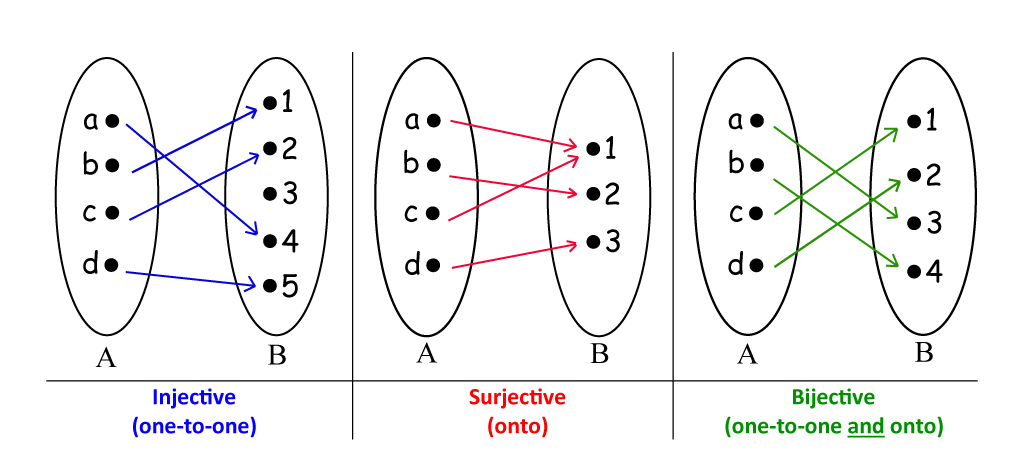
\includegraphics[width=0.9\linewidth]{images/injective-surjective-bijective.png}
    \caption{Examples of injective, surjective and bijective}
\end{figure}

\subsection{Monotone Function}
\paragraph{Definition} Let $f : D \rightarrow \mathbb{R}$ be a function.
\begin{itemize} 
     \item If $f(x_1) \leq f(x_2)$ for all $x_1$ and $x_2$ in $D$ with $x_1 < x_2$, then $f$ is
     said to be \textbf{nondecreasing or weakly increasing}.
     \item If $f(x_1) \geq f(x_2)$ for all $x_1$ and $x_2$ in $D$ with $x_1 < x_2$, then $f$ is
     said to be \textbf{nonincreasing or weakly decreasing}.
     \item  If $f(x_1) < f(x_2)$ for all $x_1$ and $x_2$ in $D$ with $x_1 < x_2$, then $f$ is
     said to be \textbf{increasing or strictly increasing}.
     \item  If $f(x_1) > f(x_2)$ for all $x_1$ and $x_2$ in $D$ with $x_1 < x_2$, then $f$ is
     said to be \textbf{decreasing or strictly decreasing}.
     \item  If $f$ is nondecreasing or nonincreasing, then $f$ is said to be
     \textbf{monotone or monotonic}.
     \item  If $f$ is (strictly) decreasing or increasing, then $f$ is said to be
     \textbf{strictly monotone or strictly monotonic}.
\end{itemize}
\subsection{Even/Odd Function}
\paragraph{Definition} Let $f : D \rightarrow \mathbb{R}$ be a function, where $D$ is a subset of $\mathbb{R}$ that is
symmetric about the origin. Then
\begin{itemize} 
    \item $f$ is called an even function if $f(-x) = f(x)$ for every $x \in D$.
    \item $f$ is called an odd function if $f(-x) = -f(x)$ for every $x \in D$.
\end{itemize}

\paragraph{Example}
The function $f(x) := x^2$ is even, while $f(x) := \sin x$ is odd (with
domain $\mathbb{R}$).

\section{Extreme Value}
\subsection{Maxima and Minima}
\paragraph{Definition}
Let $S$ be a nonempty subset of $\mathbb{R}$, and let $y \in S$. \\
We say that $y$ is a maximum of $S$ if $y \geq s$ for all $s \in S$. \\
We say that $y$ is a minimum of $S$ if $y \leq s$ for all $s \in S$. \\

\noindent
Note that not every set has an extremum. However, every nonempty finite set has a maximum and a minimum. 

\paragraph{Example}
The interval [a, b) has minimum a but no maximum, and any open interval (a, b) has
neither a maximum nor a minimum.

\subsection{Boundedness}
\paragraph{Definition} Let $S$ be a nonempty subset of $\mathbb{R}$.
\begin{itemize} 
    \item The set $S$ is said to be bounded above if there exists $u \in \mathbb{R}$
    such that $x \leq u$ for all $x \in S$. Any such number $u$ is called an
    upper bound of $S$.
    \item The set $S$ is said to be bounded below if there exists $l \in \mathbb{R}$
    such that $x \geq l$ for all $x \in S$. Any such number $l$ is called a
    lower bound of $S$.
    \item A set is said to be bounded if it is both bounded above and
    bounded below, and it is said to be unbounded otherwise.
\end{itemize}
\noindent
Note that if $S$ has one upper bound $u$, then it has infinitely many
upper bounds, e.g., u + 1, u + 2, ...

\subsection{Suprema and Infirma}
\paragraph{Definition} Let $S$ be a nonempty subset of $\mathbb{R}$. A real number $x$ is called the
supremum of $S$ (or the least upper bound of $S$) and write $x$ = sup $S$, if 
\begin{enumerate}[i] 
    \item $x$ is an upper bound of $S$, and;
    \item Let $u$ is a set of upper bound of $S$ then for every $u$, $x \leq u$.
\end{enumerate}
Similarly, we call $x$ the infirmum of $S$ (or the greatest lower bound of $S$), and write $x$ = inf $S$, if
\begin{enumerate}[i] 
    \item $x$ is an lower bound of $S$, and;
    \item Let $l$ is a set of lower bound of $S$ then for every $l$, $x \geq l$.
\end{enumerate}
By definition, there cannot be two different suprema or two different infirma for the same set. \\ \\
The supremum and the infirmum of $S$ do not have to belong to $S$ even if they exist.
For example, if $S$ = $\{1/n : n \in \mathbb{N}^+\}$, then sup $S$ = 1 and
inf $S$ = 0, so $S$ contains its supremum but not its infirmum. \\ \\
If sup $S \in S$, then sup $S$ = max $S$. Similarly, if
inf $S \in S$, then inf $S$ = min $S$. 

\begin{theorem}[Least-Upper-Bound Property of $\mathbb{R}$]
    Every nonempty set of real numbers that is bounded above has a
    least upper bound.
\end{theorem}
\begin{theorem}[Greatest-Lower-Bound Property of $\mathbb{R}$]
    Every nonempty set of real numbers that is bounded below has a
    greatest lower bound.
\end{theorem}
\end{document}
